\documentclass{protokol}
\leftheader{Metody skenovací elektronové mikroskopie (SEM)}
% \centerheader{Praktikum IV}
\rightheader{Tomáš Derner}

\begin{document}

  \section*{Úkol}

    \begin{enumerate}
      \item Studium lomových ploch pomocí SEM.
      \item Měření střední velikosti zrna polykrystalického vzorku. K vyhodnocení snímku ze skenovacího elektronového mikroskopu použijte kruhovou metodu.
      \item Určení frakčního objemu dané fáze ve vícefázovém materiálu. Použijte specializované programové vybavení pro obrazovou analýzu.
    \end{enumerate}

  \section*{Teorie}

    Skenovací elektronový mikroskop vytváří zvětšený obraz vzorku pomocí ostře fokusovaného svazku elektronů. Emitované (primární) elektrony jsou urychlovány a a vychylovacími cívkami usměrňovány na konkrétní místo na vzorku. Elektronový paprsek přejíždí po řádcích vzorek a budí odezvu, která je snímána detektory.

    Primární elektrony se ve vzorku pružně a nepružně rozptylují. Při pružném rozptylu mění elektrony pouze směr pohybu bez ztráty energie. Tyto zpětně odražené elektrony jsou následně snímány detektorem. Při nepružném rozptylu předávají primární elektrony energii volným elektronům ve vzorku a tím je excitují. V důsledku toho vznikají sekundární elektrony a gamma záření. 

    V této úloze využijeme detekci zpětně odražených elektronů, jejichž intenzita závisí na chemickém složení vzorku, a sekundárních elektronů pro pozorování topografie vzorku.

    \subsection*{Lomové plochy}

      V úloze jsou studovány vzorky intermetalické slitiny Fe\textsubscript{3}Al. Jeden ze vzorků byl tahem deformován při pokojové teplotě, druhý při teplotě $\SI{700}{\celsius}$. Plasticita slitiny Fe\textsubscript{3}Al s teplotou roste, z lomových ploch těchto vzorků je možné nahlédnout důvod.

    \subsection*{Velikost zrna}

      Běžné kovy jsou složeny z jednolitých krystalů (zrn) s různou krystalografickou orientací. Různou orientaci zrn dobře zviditelní metoda zpětně odražených elektronů, protože jsou-li krystalové plochy kolmé k řezu, pronikají elektrony hlouběji do struktury vzorku a méně se jich vrátí do detektoru. V opačném případě je intenzita zpětně odražených elektronů větší.

      Velikost zrna měříme kruhovou metodou. Ve snímku řezu vytvoříme kružnici a střední velikost zrna určíme podle vztahu
      \begin{equation} \label{eq:d}
        d = \frac{3 \pi}{2} \frac{D}{n},
      \end{equation}
      kde $D$ je průměr kružnice a $n$ počet proťatých zrn.

    \subsection*{Frakční objem druhé fáze}

      Čím větší je atomové číslo atomů ve vzorku, tím větší je intenzita zpětně odražených elektronů. Toho lze využít k určení frakčního objemu druhé fáze vícefázové slitiny určením poměru ploch fází ve vzorku.
    
  \section*{Výsledky}

    Obrázek \ref{fig:v1} zobrazuje lomové plochy vzorku deformovaného při pokojové teplotě získané pomocí metody sekundárních elektronů, na obrázku \ref{fig:v2} je zobrazeno lomové rozhraní vzorku deformovaného při teplotě $\SI{700}{\celsius}$. Je zřejmé, že při deformaci při pokojové teplotě se od sebe oddělila jednotlivá zrna, materiál má tedy slabá místa ve styku zrn, zatímco při teplotě $\SI{700}{\celsius}$ je struktura zrn nerozeznatelná, materiál je pospolitější, lépe se deformuje. Ve vzorku vznikají kavity, které nakonec způsobí lom.

    \begin{figure}[H]
      \centering 
      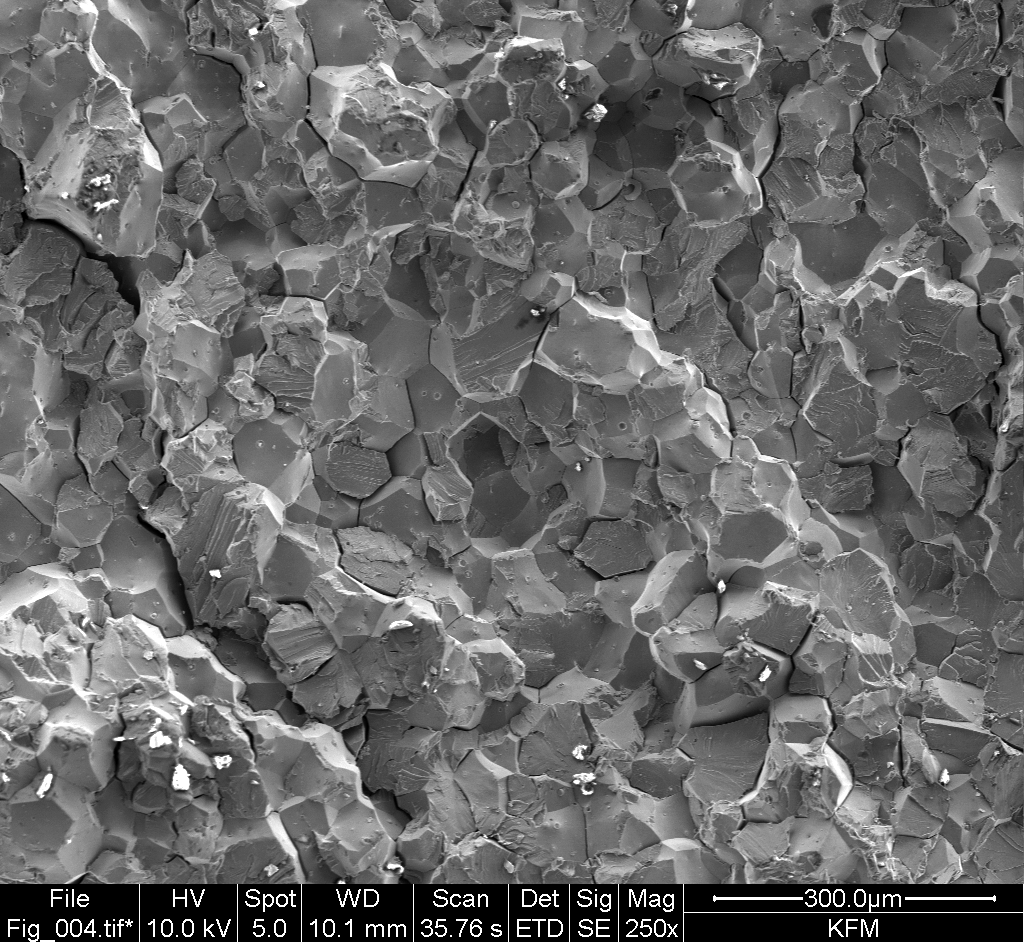
\includegraphics[width=\textwidth]{v1}
      \vspace{5pt}
      \caption{Vzorek deformovaný při pokojové teplotě}
      \label{fig:v1}
    \end{figure}

    \begin{figure}[H]
      \centering 
      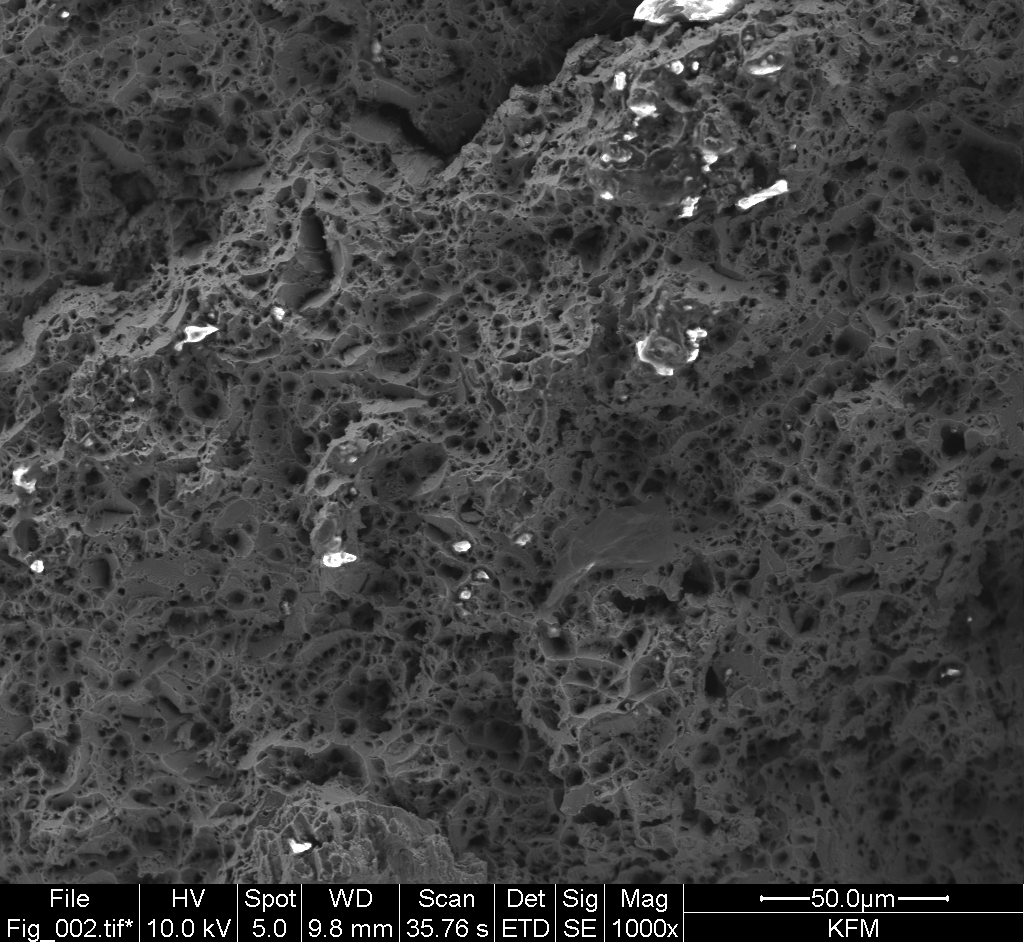
\includegraphics[width=\textwidth]{v2}
      \vspace{5pt}
      \caption{Vzorek deformovaný při teplotě $\SI{700}{\celsius}$}
      \label{fig:v2}
    \end{figure}

    \subsection*{Úkol 2}

      Byly vytvořeny čtyři snímky povrchu vzorku na různých místech pomocí zpětně odražených elektronů. Snímky byly zpracovány kruhovou metodou. Průměr použitých kružnic činí 
      $$ D = \SI{420}{\micro\metre}, $$
      kružnice protínají v jednotlivých snímcích 65, 51, 59 a 53 zrn s chybou 5 zrn. Průměrná hodnota činí
      $$ n = \num{57.0 \pm 5.9}. $$

      Podle vztahu \eqref{eq:d} je střední velikost zrna 
      $$ d = \SI{35 \pm 4}{\micro\metre}. $$


      \begin{figure}[H]
        \centering
        \hspace*{-60pt}   
        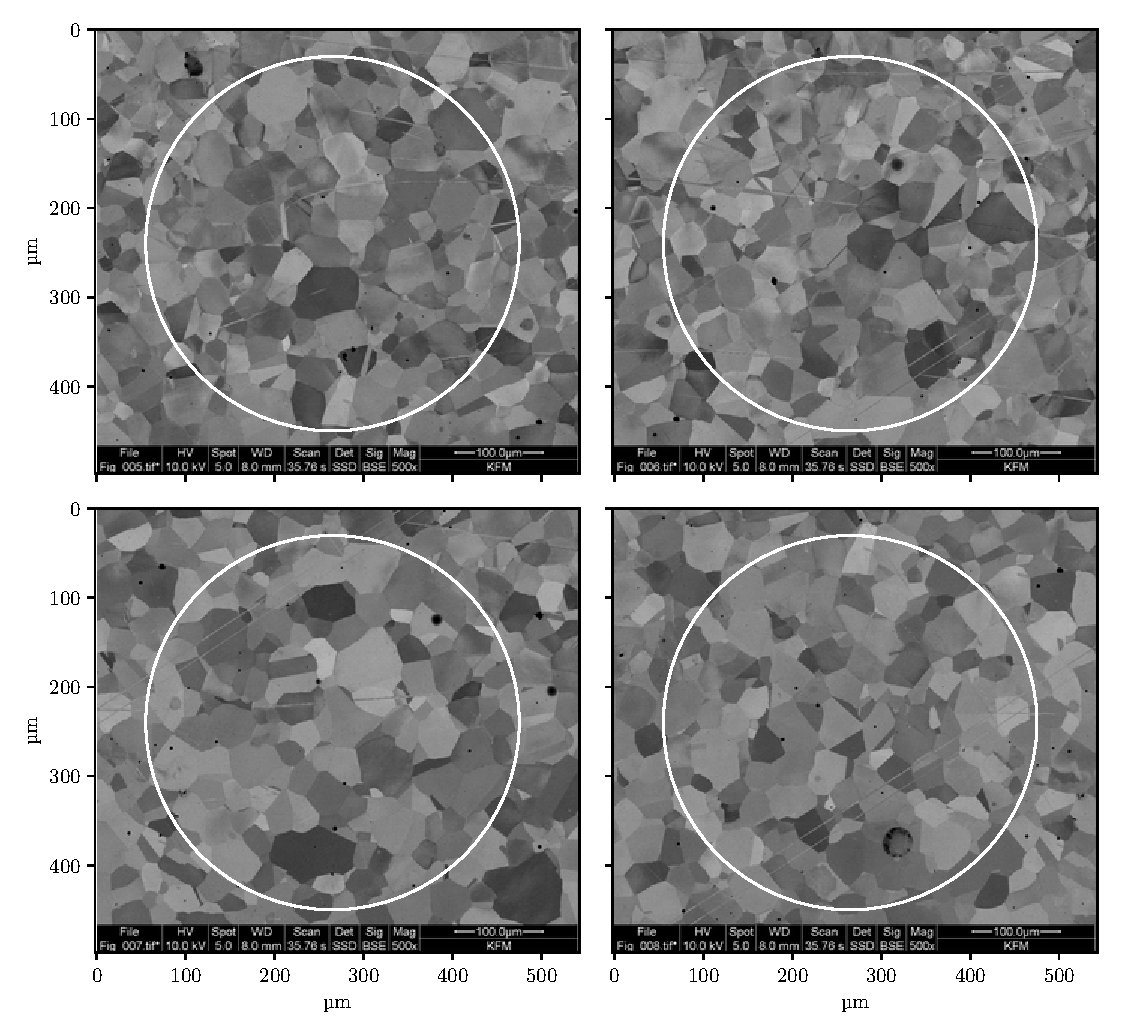
\includegraphics[]{kruh}
        \hspace*{60pt}
        \vspace{-15pt}
        \caption{Čtyři snímky z různých míst vzorku s vyznačenými kružnicemi}
        \label{fig:kruh}
      \end{figure}

    \subsection*{Úkol 3}

      Vytvořili jsme čtyři snímky vzorku slitiny cínu a olova pomocí zpětně odražených elektronů. Protože má olovo větší atomové číslo, na snímcích je tmavší než cín. V tabulce \ref{tab:u3} uvádíme poměry barev odpovídajících jednotlivým komponentám ve snímcích, v sloupci 5 a 6 pak procentuální obsah cínu a olova ve vzorku bez nečistot. Použité snímky jsou zobrazeny na obrázku \ref{fig:u3}. Chyba určení obsahu nečistot činí $\SI{0.5}{\percent}$, chyba určení obsahu cínu a olova je $\SI{3}{\percent}$.

      \begin{table}[H]
        \centering
        \setlength{\tabcolsep}{10pt}
        \begin{tabular}[t]{
  S[table-format=1.0]
  S[table-format=2.1]
} \toprule
{$d$}  & {$I$}  \\
{[cm]} & {[nA]} \\ \midrule
     2 & 6.9 \\
     3 & 10.5 \\
     4 & 12.5 \\
     5 & 12.5 \\
     6 & 12.5 \\ \bottomrule
\end{tabular}
        \caption{Tabulka obsahu komponent ve vzorku}
        \label{tab:u3}
      \end{table}

      \vspace{-8pt}
      
      \begin{figure}[H]
        \centering
        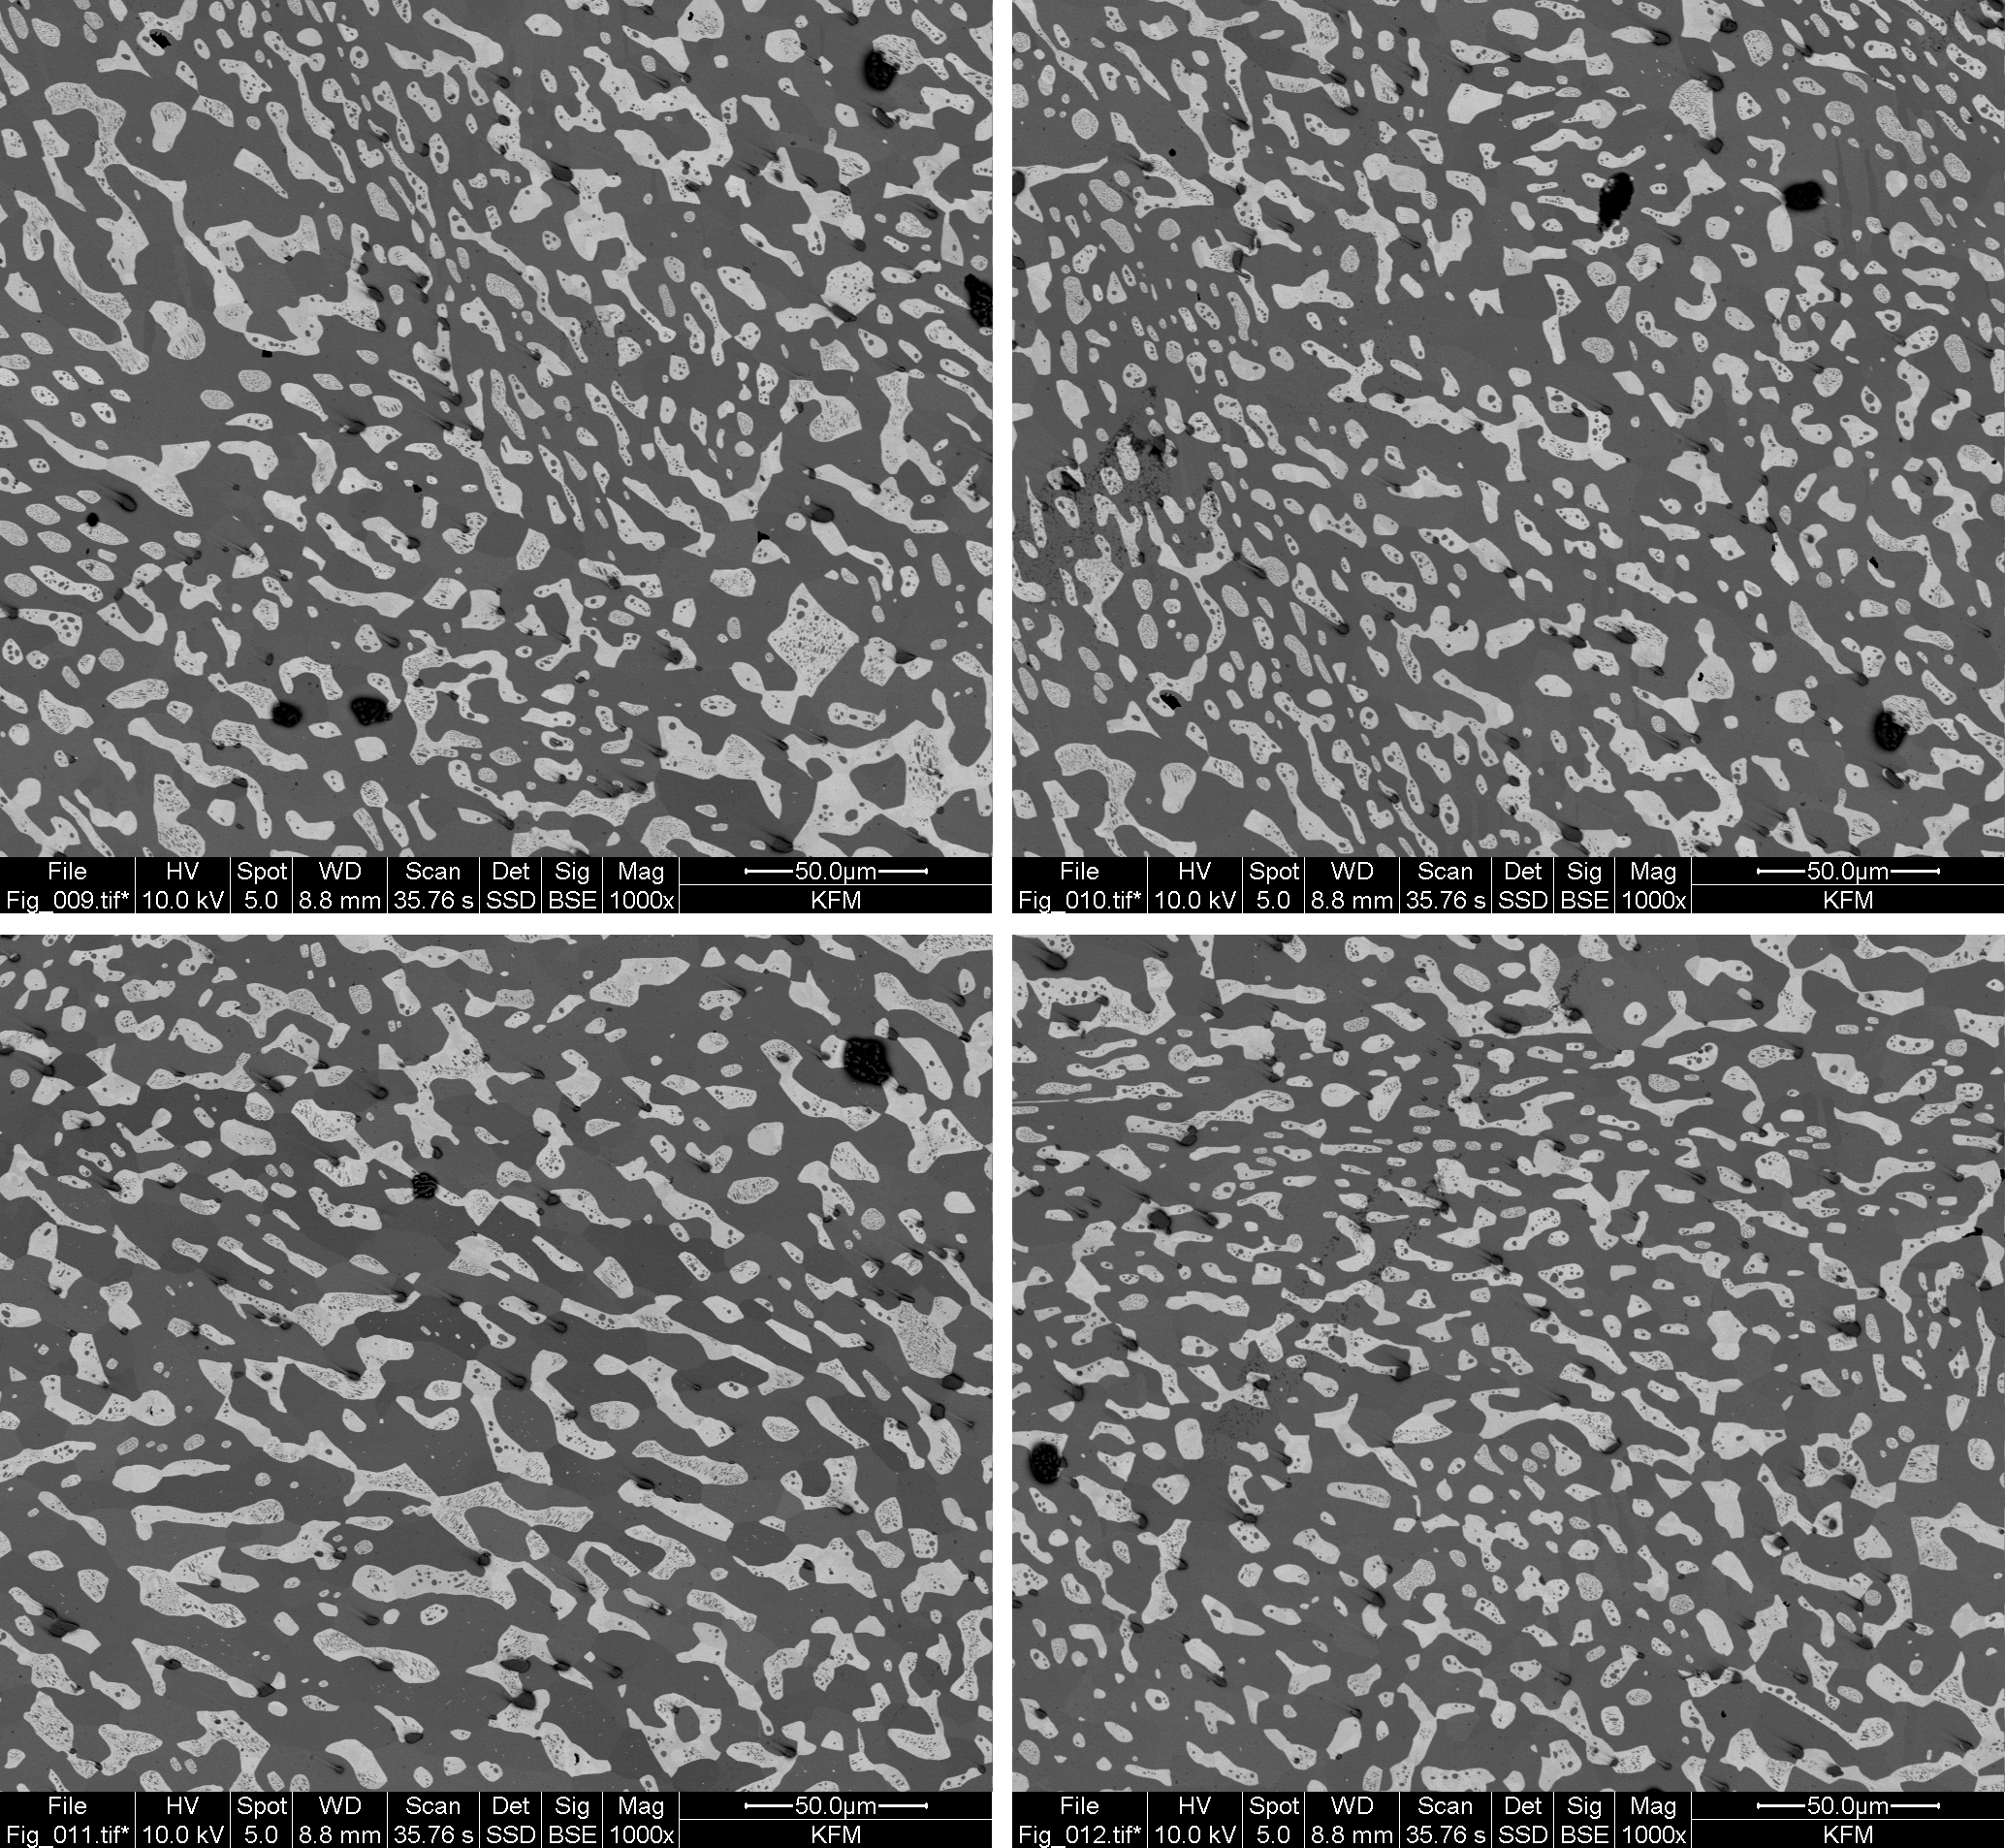
\includegraphics[width=\textwidth]{u3}
        \vspace{5pt}
        \caption{Čtyři snímky povrchu vzorku slitiny cínu a olova}
        \label{fig:u3}
      \end{figure}
      \vspace{-10pt}
      
      Aritmetickým průměrem dostaneme poměr obsahu cínu a olova ve vzorku bez nečistot 
      $$ \text{obsah cínu} = \SI{70.1 \pm 3.0}{\percent}, $$ 
      $$ \text{obsah olova} = \SI{29.9 \pm 3.0}{\percent}. $$

  \section*{Diskuse}

    Hodnota střední velikosti zrna je zatížena značnou chybou, protože v některých případech není jednoduché rozlišit hranice jednotlivých zrn. 

    Ačkoliv jsou určené poměry barev odpovídajících jednotlivým komponentám slitiny relativně blízko sebe a tudíž netrpí přílišnou statistickou chybou, neurčitost v metodě měření nutí odhadnout chybu poměrně vysoko. Barvy totiž nejsou zcela jednolité a určení rozhraní mezi dvěma komponentami je značně závislé na rozhodnutí experimentátora.


  \section*{Závěr}

    Byly pozorovány lomové plochy dvou vzorků Fe\textsubscript{3}Al, snímky byly přiřazeny ke vzorkům a byla kvalitativně vysvětlena křehkost materiálu při pokojové teplotě a vyšší pružnost při teplotě $\SI{700}{\celsius}$. 

    Ze čtyř snímků vzorku byla určena střední velikost zrna materiálu 
    $$ d = \SI{35 \pm 4}{\micro\metre}. $$

    Byly určeny poměry obsahu cínu a olova ve slitině bez nečistot
    $$ \text{obsah cínu} = \SI{70.1 \pm 3.0}{\percent}, $$ 
    $$ \text{obsah olova} = \SI{29.9 \pm 3.0}{\percent}. $$


  \begin{thebibliography}{}
 
    \bibitem{pokyny}
    Pokyny k měření ``Určení strukturních parametrů krystalických látek metodami skenovací elektronové mikroskopie (SEM)'', dostupné z\\ \url{https://physics.mff.cuni.cz/vyuka/zfp/_media/zadani/texty/txt_418.pdf}, 13.\,11.\,2018
   
  \end{thebibliography}

\end{document} 